

\documentclass{article}

\usepackage{fullpage,latexsym,picinpar,amsmath,amsfonts,graphicx}

\input{macros.tex}

\begin{document}
\centerline{REMOVED}
\centerline{REMOVED}
\centerline{\large \bf CS/MATH111 ASSIGNMENT 3}
%\centerline{due Wednesday, May 15}

\vskip 0.2in
%\noindent{\bf Individual assignment:} Problems 1 and 2.

%\noindent{\bf Group assignment:} Problems 1,2 and 3.

\vskip 0.1in

%%%%%%%%%%%%%%%%%%%%%%%%%%%%

\newcommand{\ttA}{\texttt{A}}
\newcommand{\ttB}{\texttt{B}}
\newcommand{\ttC}{\texttt{C}}
\newcommand{\ttE}{\texttt{E}}
\newcommand{\ttF}{\texttt{F}}

\begin{problem}
Strings of length $n$ are composed of the following strings: $\tt1$, $\tt2\tt2$, $\tt2\tt3$, $\tt3\tt2$, $\tt3\tt3$,
$\tt4\tt4\tt5$ and $\tt5\tt4\tt4$. Let $S_n$ be the number of strings of length $n$ that can
be formed in this way. For example, for $n=3$, we can form the following strings:
%
\begin{align*}
\tt1\tt1\tt1
,
\tt1\tt2\tt2  , \tt1\tt2\tt3  , \tt1\tt3\tt2  , \tt1\tt3\tt3
,
\tt2\tt2\tt1  , \tt2\tt3\tt1  , \tt3\tt2\tt1  , \tt3\tt3\tt1 
,
\tt4\tt4\tt5 , \tt5\tt4\tt4
\end{align*}
%
and thus $S_3 = 11$. (Note that $S_0 = 1$, because the
empty string satisfies the condition.)

\smallskip
\noindent (a) Derive a recurrence relation for the numbers $S_n$. Justify it.

\smallskip
\noindent (b) \textbf{Extra credit}. Let $P_n$ be the number of strings of length $n$ that can
be formed from the given strings,  considering that four 1's cannot be next to each other. (The substring 1111 is not allowed.) Derive a recurrence relation for the numbers $P_n$. Justify it.
\smallskip
%\noindent (b) Find the formula for the numbers $S_n$ by solving this recurrence. Show your work.
\end{problem}

\smallskip
%%%%%%%%%%%%%%%%%%%%%%%%%%%%
\begin{solution}
\newline
a.) Let $S_n$ be the number of strings of length $n$ that can be formed in this way.

\begin{center}
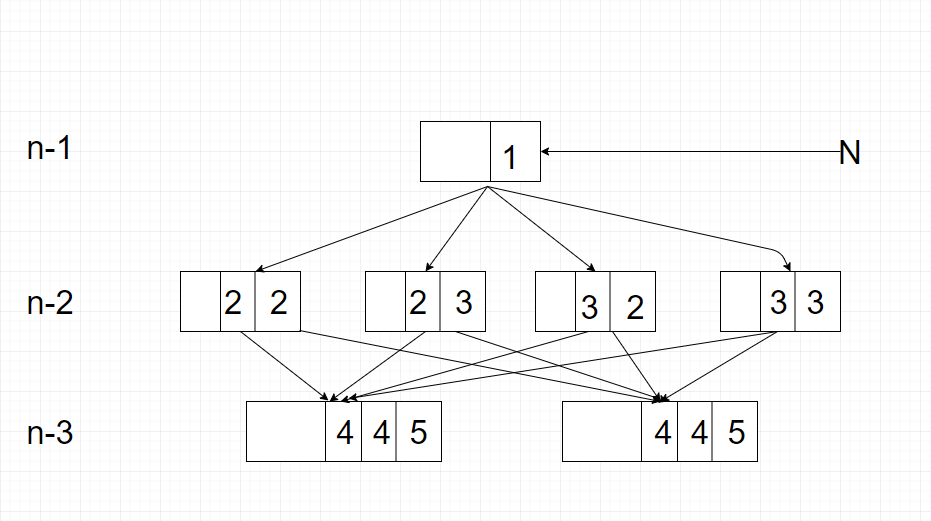
\includegraphics[width=4in]{diagram.PNG}
\newline
\end{center}

We have one possible string of size one, which is the first box at the top. This is denoted as $S_{(n-1)}$. We then have four possible strings of size two, which is denoted as 4$S_{(n-2)}$ and are the boxes represented in the middle. We finally have two strings of size three, which is denoted as $2S_{(n-3)}$ and are the boxes represented on the bottom.

We then have three initial conditions to work with:
\newline
$S_0 = 1$
This is from the empty string condition that must satisfy the equation.
\newline
$S_1 = 1$
This is from the first box, where we would have the single variable string of 1.
\newline
$S_2 = 5$
This is from having the four strings of 2 and adding in the single 1 char string.
\newline
We are then given the following condition:
\newline
$S_3 = 11$.

Therefore, with the information we have, we get the recurrence relation for $S_n$ of:
\newline
$S_n=S_{(n-1)} + S_{(n-2)} + S_{(n-3)}$
\newline

b.) We are letting $P_n$ be the number of strings of length $n$ that can be formed from the original given strings. However, we cannot allow four 1's to be next to each other. With not having four single strings next to each other, we would have to subtract the situation of $S_{(n-4)}$. So, the solution would be:
\newline
$P_n=S_{(n-1)} + S_{(n-2)} + S_{(n-3)}-S_{(n-4)}$




\end{solution}
%%%%%%%%%%%%%%%%%%%%%%%%%%%%

\begin{problem}
Solve the following recurrence equation:
\smallskip
\begin{align*}
	S_n &= S_{n-1} + 4S_{n-2} + 2S_{n-3}
	\\
	S_0 &= 1
	\\
	S_1 &= 1
	\\
	S_2 &= 5
\end{align*}

\noindent Show your work (all steps: the characteristic polynomial and its roots, the general solution, 
using the initial conditions to compute the final solution.)
\end{problem}

%%%%%%%%%%%%%%%%%%%%%%%%%%%%
\begin{solution}

Characteristic Equation: $x^{3} - x^{2} -4x - 2 = 0$

\smallskip
$(-1)^{3} - (-1)^{2} - 4(-1) -2 = -1 - 1 + 4 - 2 = 0$
\smallskip

So $r_1 = -1$ and $(x+1)$ is a factor
\smallskip

$\frac{x^{3} - x^{2} - 4x - 2}{x + 1} = x^2 - 2x - 2$
\smallskip

$r_2 = \frac{2 + \sqrt{4 + 8}}{2} = 1 + \sqrt{3}$

$r_3 = 1 - \sqrt{3}$

\smallskip
General Solution: $S_n = \alpha_1(-1)^{n} + \alpha_2(1 + \sqrt{3})^{n} + \alpha_3(1 - \sqrt{3})^{n}$

\smallskip
Using the Initial Conditions: 

%\begin{align*}
\begin{flalign}
      &  1 = \alpha_1 + \alpha_2 + \alpha_3 \\
      &  1 = -\alpha_1 + \alpha_2(1 + \sqrt{3}) + \alpha_3(1 - \sqrt{3}) \\
      &  5 = \alpha_1 + \alpha_2(1 + \sqrt{3})^{2} + \alpha_3(1 - \sqrt{3})^{2}
%\end{align*}
\end{flalign}

Adding equations (1) and (2) we get:
\begin{flalign}
    & 2 = \alpha_2 + \alpha_2(1 + \sqrt{3}) + \alpha_3 + \alpha_3(1 - \sqrt{3}) \nonumber \\
    & 2 = \alpha_2(1 + (1 + \sqrt{3})) + \alpha_3(1 + (1 - \sqrt{3})) \nonumber \\
    & 2 = \alpha_2(2 + \sqrt{3}) + \alpha_3(2 - \sqrt{3}) 
\end{flalign}

Adding equations (2) and (3) we get :
\begin{flalign}
    & 6 = \alpha_2(1 + \sqrt{3}) + \alpha_2(1 + \sqrt{3})^{2} + \alpha_3(1 - \sqrt{3})^{2} + \alpha_3(1 - \sqrt{3})^2 \nonumber \\
    & 6 = \alpha_2((1+\sqrt{3}) + (1 + 2\sqrt{3} +3)) + \alpha_3((1-\sqrt{3}) + (1 - 2\sqrt{3} + 3)) \nonumber \\
    & 6 = \alpha_2(5 + \sqrt{3}) + \alpha_3(5 - \sqrt{3})
\end{flalign}

Multiplying (5) by $2+\sqrt{3}$ and (4) by $5+\sqrt{3}$ and subtracting we get:
\begin{flalign}
    & 6(2 + \sqrt{3}) - 2(5 + \sqrt{3}) = \alpha_3(5-\sqrt{3})(2+\sqrt{3}) - \alpha_3(2-\sqrt{3})(5+\sqrt{3}) \nonumber \\
    & 12 + 6\sqrt{3} - 10 - 6\sqrt{3} = \alpha_3((5-3\sqrt{3})(2+\sqrt{3}) - (2-\sqrt{3})(5+3\sqrt{3})) \nonumber \\
    & 2 = \alpha_3((10+5\sqrt{3}-6\sqrt{3}-9)-(10+6\sqrt{3}-5\sqrt{3}-9)) \nonumber \\
    & 2 = \alpha_3(10\sqrt{3} - 12\sqrt{3}) = \alpha_3(-2\sqrt{3}) \nonumber \\
    & \alpha_3 = -\frac{1}{\sqrt{3}} \nonumber
\end{flalign}

Plugging $\alpha_3$ into (4) we get:
\begin{flalign}
    & 2 = \alpha_2(2+\sqrt{3}) + (-\frac{1}{\sqrt{3}}) \nonumber \\
    & 2 = \alpha_2(2+\sqrt{3}) - \frac{2}{\sqrt{3}} + 1 \nonumber \\
    & \alpha_2 = \frac{1 + \frac{2}{\sqrt{3}}}{2 + \sqrt{3}} \nonumber \\
    & \alpha_2 = \frac{\frac{\sqrt{3}}{\sqrt{3}}+\frac{2}{\sqrt{3}}}{2+\sqrt{3}} = \frac{1}{\sqrt{3}} \nonumber
\end{flalign}

Plugging $\alpha_2$ and $\alpha_3$ into (1) and solving for $\alpha_1$ we get: \newline

\centerline{$\alpha_1 = 1 - \frac{1}{\sqrt{3}} + \frac{1}{\sqrt{3}} = 1$} 

\smallskip\smallskip\smallskip

Final Solution: $S_n = (-1)^{n} + \frac{1}{\sqrt{3}}(1+\sqrt{3})^{n} - \frac{1}{\sqrt{3}}(1-\sqrt{3})^{n}$
\end{solution}


%%%%%%%%%%%%%%%%%%%%%%%%%%%%
\begin{problem}
Solve the following recurrence equation:
%
\begin{eqnarray*}
        D_n &=& 4D_{n-1} -8 D_{n-3} + 2n+3\\
        D_0 &=& 0 \\
        D_1 &=& 1 \\
		D_2 &=& 1
\end{eqnarray*}
%
Show your work (all steps: the associated homogeneous equation,
the characteristic polynomial and its
roots, the general solution of the homogeneous
equation, computing a particular solution,
the general solution of the non-homogeneous equation,
using the initial conditions to compute the final solution.)
\end{problem}

%%%%%%%%%%%%%%%%%%%%%%%%%%%%
\begin{solution}

Associated Homogeneous equation: $D_{nc}=4D_{n-1} - 8D_{n-3}$

\smallskip
Characteristic Equation: $x^{3} - 4x^{2} - 8 = 0$

\smallskip
$(2)^{3} - 4(2)^{2} + 8 = 0$

\smallskip
So $r_1=2$ and (x-2) is a factor

\smallskip
$(x-2)(x^{2}-2x-4) = 0$

\smallskip
Roots: $r_2 = 1+\sqrt{5}$, $r_3 = 1-\sqrt{5}$

\smallskip
General homogeneous solution: $D'_n = \alpha_12^{n} + \alpha_2(1+\sqrt{5})^{n} + \alpha_3(1-\sqrt{5})^{n}$

\smallskip
Assume a particular solution has the form $p_1n + p_0$
\begin{flalign}
    & p_1n + p_0= 4(p_1(n-1)+p_0) - 8(p_1(n-3)+p_0) + 2n + 3 \nonumber \\
    & n(2-5p_1) + (20p_1-5p_0) + 3 = 0 \nonumber \\
    & p_1 = \frac{2}{5} \nonumber \\
    & p_0 = \frac{11}{5} \nonumber
\end{flalign}

Particular Solution: $D''_n = \frac{2}{5}n + \frac{11}{5}$
 
\smallskip
General Non-homogeneous Solution: $D_n = D'_n + D''_n = \alpha_12^{n} + \alpha_2(1+\sqrt{5})^{n} + \alpha_3(1-\sqrt{5})^{n} + \frac{2}{5}n + \frac{11}{5}$

\smallskip
Using the initial Conditions:
\begin{flalign}
    & 0 = \alpha_1 + \alpha_2 + \alpha_3 + \frac{11}{5} \nonumber \\
    & 1 = 2\alpha_1 + \alpha_2(1+\sqrt{5}) + \alpha_3(1-\sqrt{5} + \frac{9}{5}\nonumber \\
    & 1 = 4\alpha_1 + \alpha_2(1+\sqrt{5})^{2} + \alpha_3(1-\sqrt{5})^{2} +3 \nonumber 
\end{flalign}

Solving the system of equations we find:
\begin{flalign}
    & \alpha_1 = -\frac{5}{2} \nonumber \\
    & \alpha_2 = \frac{15+31\sqrt{5}}{100} \nonumber \\
    & \alpha_3 = \frac{15-31\sqrt{5}}{100} \nonumber 
\end{flalign}

Final Solution: $D_n = (-\frac{5}{2})2^{n} + (\frac{15+31\sqrt{5}}{100})(1+\sqrt{5})^{n} + (\frac{15-31\sqrt{5}}{100})(1-\sqrt{5})^{n} + \frac{2}{5}n + \frac{11}{5}$

\end{solution}
%%%%%%%%%%%%%%%%%%%%%%%%%%%%
\begin{problem}
Solve the following recurrence equation:
%
\begin{eqnarray*}
        A_n &=& A_{n-1} + 2A_{n-2} + 3^n\\
        A_0 &=& 0 \\
        A_1 &=& 4
\end{eqnarray*}
%
Show your work (all steps: the associated homogeneous equation,
the characteristic polynomial and its
roots, the general solution of the homogeneous
equation, computing a particular solution,
the general solution of the non-homogeneous equation,
using the initial conditions to compute the final solution.)
\end{problem}

%%%%%%%%%%%%%%%%%%%%%%%%%%%%

\begin{solution}

Associated homogeneous equation: $A_{nc} = A_{n-1} + 2A_{n-2}$

\smallskip
Characteristic Equation: $x^{2} - x - 2 = (x-2)(x+1) = 0$

\smallskip
Roots: $r_1=2$, $r_2 = -1$

\smallskip
General Homogeneous Solution: $A'_n = \alpha_12^{n} + \alpha_2(-1)^{n}$

\smallskip
We assume $A_n$ has a particular solution in the form $c3^{n}$

\smallskip
Plug $c3^{n}$ into $A_n$, divide by $3^{n-2}$ and solve for $c$: 
\begin{flalign}
    & c3^{n} = c3^{n-1} + 2c3^{n-2} + 3^{n} \nonumber \\
    & 9c = 3c + 2c + 9 \nonumber \\
    & c = \frac{9}{4} \nonumber
\end{flalign}

Particular Solution: $A''_n = (\frac{9}{4})3^{n}$

\smallskip
General Non-homogeneous Solution: $A_n = A'_n + A''_n =  \alpha_12^{n} + \alpha_2(-1)^{n} + (\frac{9}{4})3^{n}$

\smallskip
Using the Initial conditions:
\begin{flalign}
    & 0 = \alpha_1 + \alpha_2 + \frac{9}{4} \nonumber \\
    & 4 = 2\alpha_1 - \alpha_2 + \frac{27}{4} \nonumber \\
    & 4 = 3\alpha_1 + 9 \nonumber \\
    & \alpha_1 = -\frac{5}{3} \nonumber \\
    & \alpha_2 = \frac{5}{3} - \frac{9}{4} = -\frac{7}{12} \nonumber
\end{flalign}

Final Solution: $A_n = (-\frac{5}{3})2^{n} - \frac{7}{12}(-1)^{n} + (\frac{9}{4})3^{n}$


\end{solution}

%%%%%%%%%%%%%%%%%%%%%%%%%%%%

\vskip 0.1in
\paragraph{Submission.}
To submit the homework, you need to upload the pdf file into gradescope and iLearn.

\end{document}

